\chapter{Impostazione del problema di ricerca}
\label{FormulazioneProblema}
\thispagestyle{empty}

%\begin{quotation}
%{\footnotesize
%\noindent{\emph{``Terence: Rotta a nord con circospezione \\
%Bud: Ehi, gli ordini li do io qui!\\
%Terence: Ok, comante\\
%Bud: Rotta a nord\\
%Terence: Soltanto?\\
%Bud: Con circospezione!''}
%}
%\begin{flushright}
%Chi Trova un Amico Trova un Tesoro
%\end{flushright}
%}
%\end{quotation}
\vspace{0.5cm}
In questo capitolo descriviamo il problema affrontato dall'algoritmo di tampering detection, in maniera formale e rigorosa. \\
Nel Paragrafo \ref{modelloOsservaz} illustriamo il modello delle osservazioni e gli eventi che siamo interessati a identificare.\\
Nel Paragrafo \ref{tamperingDef} formalizziamo il concetto di tampering detection. 
\noindent 
\section{Modello delle osservazioni}
\label{modelloOsservaz}
Il nostro campo di osservazione si concentra su quegli eventi che si interpongono tra la scena ripresa da una camera e il sensore che acquisisce le immagini. Non vogliamo, cio\`e, identificare degli eventi particolari che avvengono nella scena, come un oggetto lasciato incustodito \cite{Targhe}, bens\`i vogliamo identificare quegli eventi che non permettano al sensore di riprendere in maniera ottimale la scena, quali ad esempio sfocature o spostamenti della camera.
Nel seguito cerchiamo di dare una definizione formale di questi eventi.
\subsection{Sfocatura}
\label{sfocatura}
Il fenomeno della sfocatura avviene quando un elemento trasparente o semitrasparente si interpone tra la lente della camera e la \gls{scena} ripresa, oppure quando viene cambiata la messa a fuoco, causando una perdita nei dettagli della \gls{scena} ripresa.

\begin{figure}[tb]
	\centering
	\begin{subfigure}[]
		{\label{fig:pioggia} 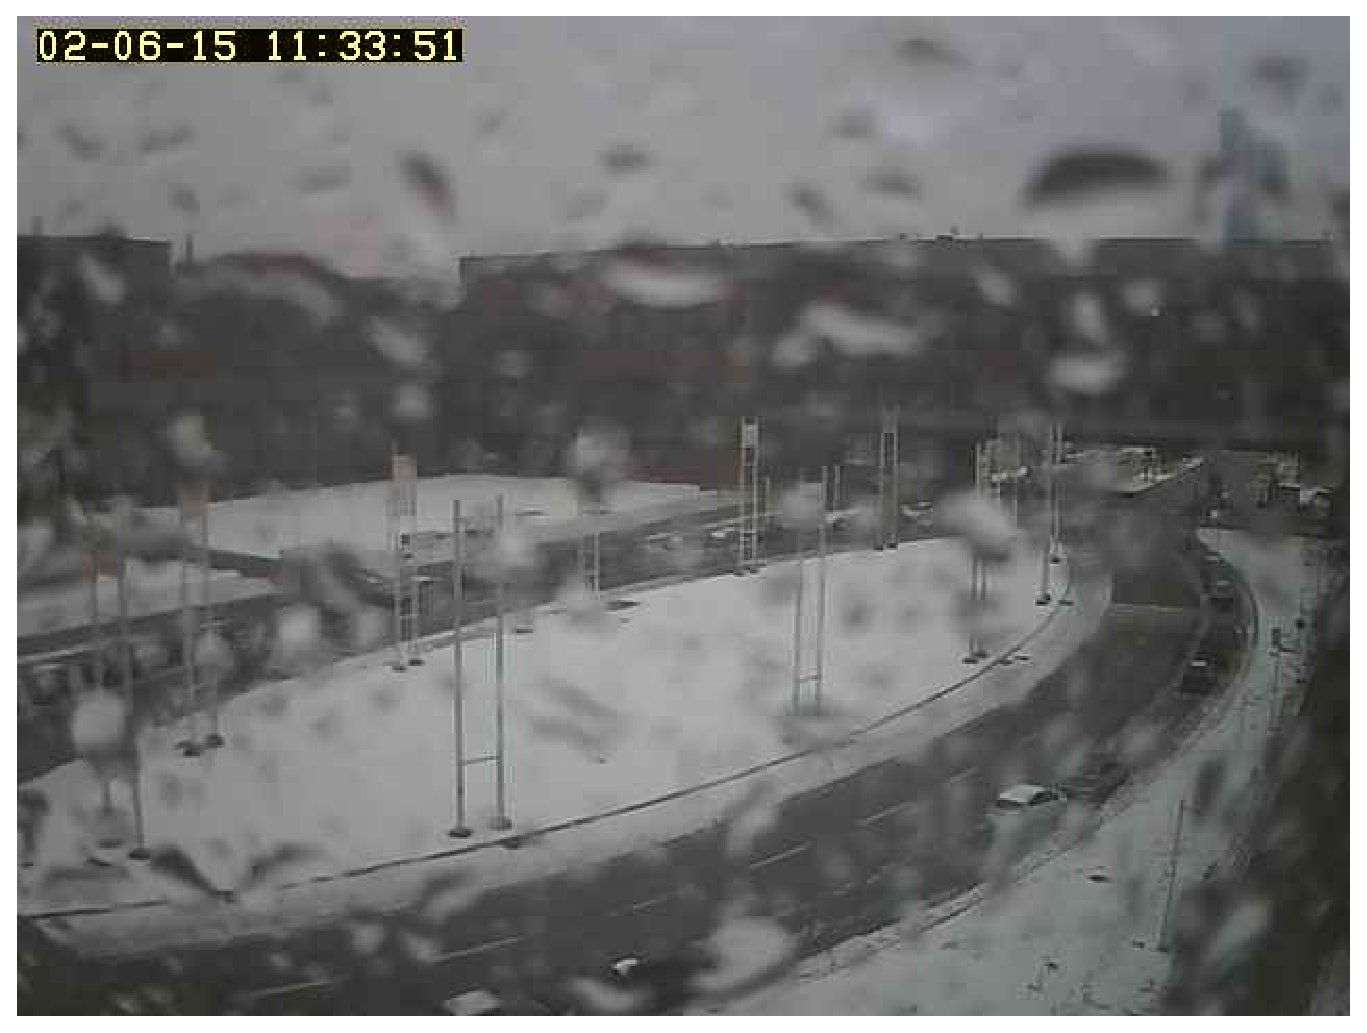
\includegraphics[width=6cm]{./pictures/pioggia}}
	\end{subfigure}
	\begin{subfigure}[]
		{\label{fig:bassiniDEFOCUS} \includegraphics[width=6cm]{./pictures/bassiniDEFOCUS}}
	\end{subfigure}
	\caption{Esempi di sfocature}
	\label{fig:esempiSfocature}
\end{figure}
\noindent Nella Figura \ref{fig:esempiSfocature} sono mostrati degli esempi in cui sono presenti delle sfocature. 
Queste possono essere di origine diversa: 
\begin{itemize}
	\item dovute a \textit{cause naturali}, come ad esempio dell'acqua piovana che si deposita sulla lente (Figura \ref{fig:pioggia}), o la condensa dovuta all'umidit\`a e alle basse temperature, oppure un raggio di sole incidente sull'obiettivo della camera;
	\item per \textit{intervento dell'uomo}, che a sua volta pu\`o avvenire in maniera intenzionale (e in questo caso si pu\`o parlare di \textit{manomissione}) oppure non intenzionale. Ad esempio, si pu\`o direttamente intervenire sulla messa a fuoco, nel caso sia possibile cambiarla manualmente; oppure (come nel caso della Figura \ref{fig:bassiniDEFOCUS}) \`e possibile applicare una sostanza semitrasparente sulla lente della camera, come il gas di un deodorante spray.
\end{itemize}
Inoltre, possiamo notare come nella Figura \ref{fig:bassiniDEFOCUS} la sfocatura riguardi tutta l'immagine, mentre nella Figura \ref{fig:pioggia} la sfocatura si concentri solo in alcune aree (quelle dove sono presenti le gocce). 
Nel primo caso si parler\`a, quindi, di sfocatura \textit{totale}, mentre nel secondo caso di sfocatura \textit{parziale}.\\
Riprendendo la trattazione presente in \cite{alippi2010detecting}, questo fenomeno pu\`o essere modellato come un operatore di \textit{degradazione} $\mathcal{D}$ applicato a un'immagine $y$, considerata priva di errori, i.e.,
\begin{equation}
z=\mathcal{D}[y].
\end{equation}
In particolare, all'interno dell'operatore $\mathcal{D}$ si pu\`o considerare il contributo dovuto a un operatore di \textit{sfocatura} $\mathcal{B}$ (dall'inglese \textit{blur}) e un termine aleatorio $\eta$ corrispondente al rumore, i.e.,
\begin{equation}
\label{blur_single}
z(x)=\mathcal{D}[y](x) = \mathcal{B}[y](x) + \eta(x), \qquad x \in \mathcal{X}
\end{equation}
dove, come abbiamo specificato nel Paragrafo \ref{concetti}, indichiamo con $x$ le coordinate dei \textit{pixel} dell'immagine e con $\mathcal{X}$ l'insieme dei pixel che formano l'immagine. 
Per praticit\`a possiamo assumere che l'operatore di blur sia \textit{lineare}.
Quindi, considerando l'immagine come un dato \textit{continuo},
\begin{equation}
\label{eq:blur}
\mathcal{B}[y](x) = \int_{\mathcal{X}}y(s)h(x,s)ds,
\end{equation}
dove $h(x,\cdot)$ rappresenta la \textit{risposta all'impulso}, \textit{point spread function} (PSF), della sfocatura sul pixel $x$.
L'effetto di $h(x, \cdot)$ \`e quello di rendere le differenze di intensit\`a, tra pixel adiacenti, pi\`u morbide (\textit{smooth}).
Nel caso in cui la sfocatura sia applicata sulla totalit\`a dell'immagine e fosse \textit{spazio invariante} (come nel caso della Figura \ref{fig:bassiniDEFOCUS}), allora \`e possibile modellare l'operatore di blur come una \textit{convoluzione}\footnote{Il blur convoluzionale \`e quello che abbiamo utilizzato per generare, in maniera sintetica, sequenze con immagini sfocate.}:
\begin{equation}
\label{blur_convolution}
\mathcal{B}[y](x) = \int_{\mathcal{X}}y(s)h(s-x)ds,
\end{equation}
dove $h(\cdot)$ \`e un filtro gaussiano o uniforme.\\
Nel caso pi\`u generale possiamo considerare che la camera acquisisca una sequenza di $N$ osservazioni (dove $N$ pu\`o tendere all'infinito) $\{z_t\}, t = 1, \dots ,N$, quindi la formula \eqref{blur_single} si pu\`o riscrivere come
\begin{equation}
\label{blur_multi}
z_t(x)=\mathcal{D}_t[y_t](x) = \mathcal{B}_t[y_t](x) + \eta(x), \qquad x \in \mathcal{X}.
\end{equation}
La sequenza delle immagini $\{y_t\}, t = 1,\dots , N$, pu\`o variare in maniera significativa nel suo contenuto, anche nel caso in cui la vista sia la stessa.
\begin{figure}[tb]
	\centering
	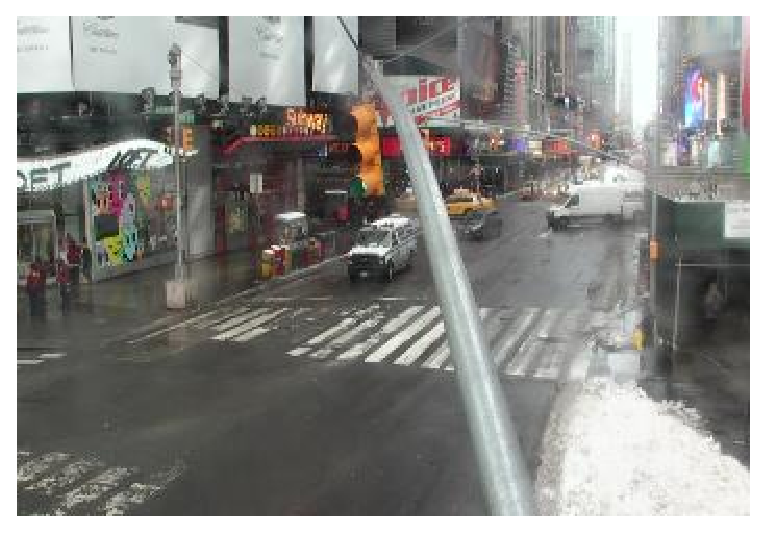
\includegraphics[width=3cm]{./pictures/image0001.eps}
	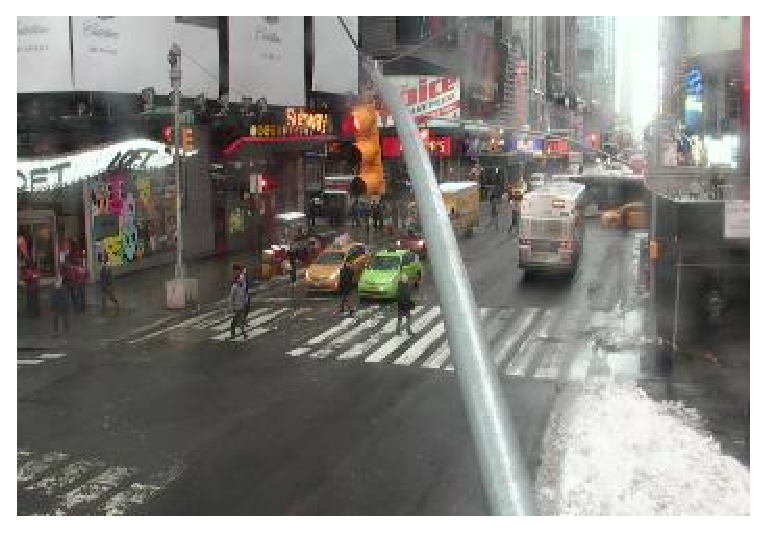
\includegraphics[width=3cm]{./pictures/image0002.eps}
	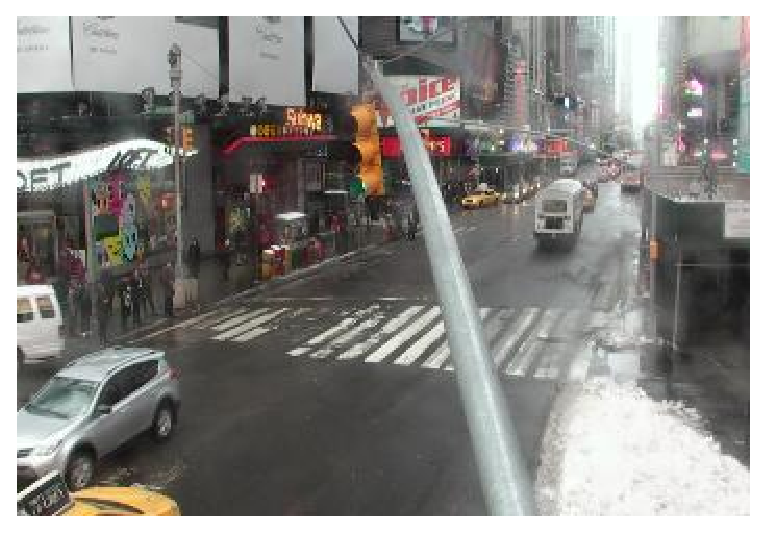
\includegraphics[width=3cm]{./pictures/image0003.eps}
	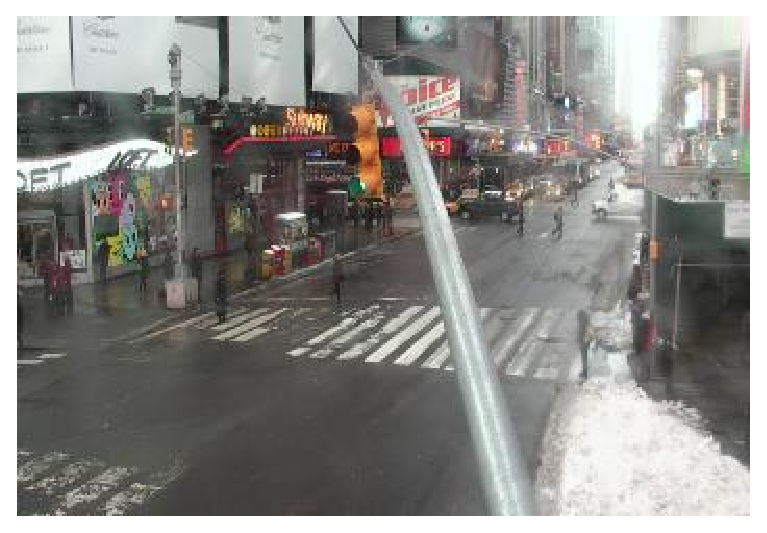
\includegraphics[width=3cm]{./pictures/image0004.eps}
	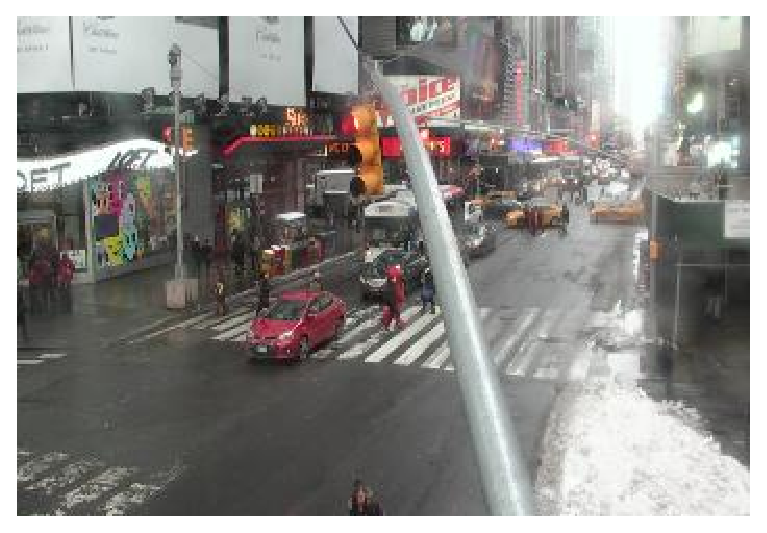
\includegraphics[width=3cm]{./pictures/image0005.eps}
	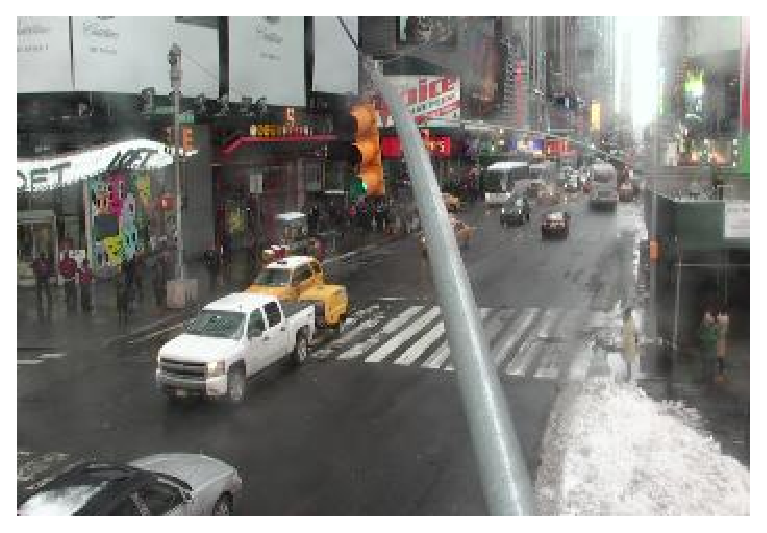
\includegraphics[width=3cm]{./pictures/image0006.eps}
	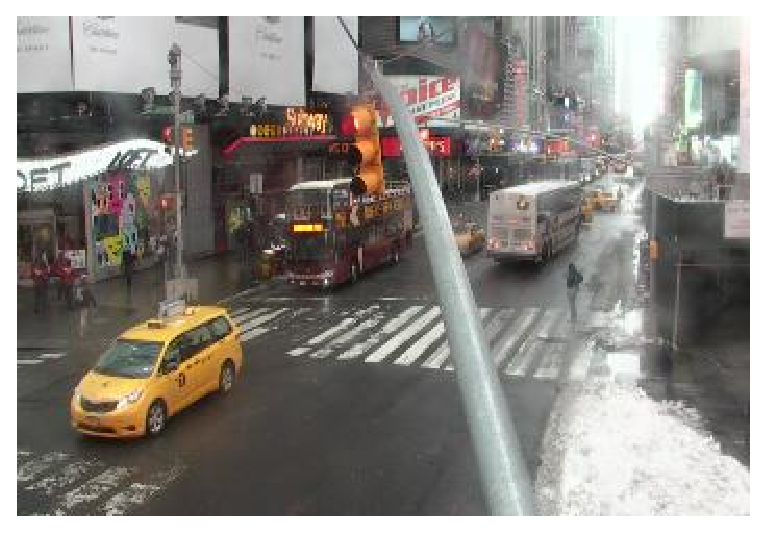
\includegraphics[width=3cm]{./pictures/image0007.eps}
	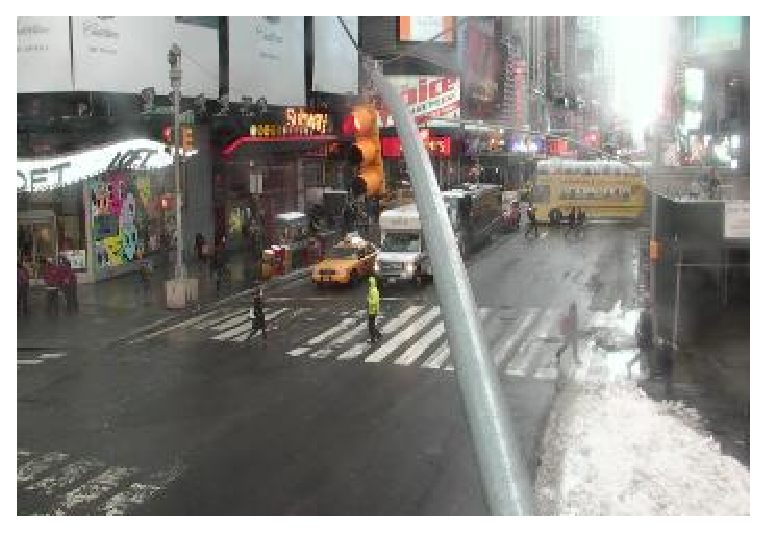
\includegraphics[width=3cm]{./pictures/image0008.eps}
	\caption{Sequenza di otto frame consecutivi acquisiti ogni minuto}
	\label{fig:framDifferences}
\end{figure}
\noindent Un esempio \`e illustrato nella Figura \ref{fig:framDifferences}, in cui le immagini riprese dalla camera sono acquisite ogni minuto. 
Nonostante l'inquadratura non cambi tra le acquisizioni, il contenuto delle singole immagini varia parecchio, a causa del continuo passaggio di automobili e pedoni.
Questo problema fa s\`i che l'identificazione delle sfocature non possa avvenire facendo un semplice confronto tra frame consecutivi, in quanto avremmo un numero troppo elevato di falsi positivi.
Infatti, nel caso in cui avessimo un riscontro negativo dal confronto tra due frame ($z_t \neq z_{t + 1}$), sarebbe difficile capire se \`e cambiato il contenuto delle immagini ($y_t \neq y_{t + 1}$) o l'operatore di sfocatura ($\mathcal{B}_t \neq \mathcal{B}_{t + 1}$). 
\subsection{Spostamento della camera}
\label{displacement}
Lo spostamento della camera avviene quando cambia la sua inquadratura.
Le cause possono essere, ancora una volta, di tipo naturale, ad esempio una raffica di vento che sposta la camera, oppure dovute a un intervento umano, uno spostamento intenzionale per evitare che la scena venga ripresa.
\begin{figure}[tb]
	\centering
	\subfigure[]{\label{fig:displacementORIGINALE} 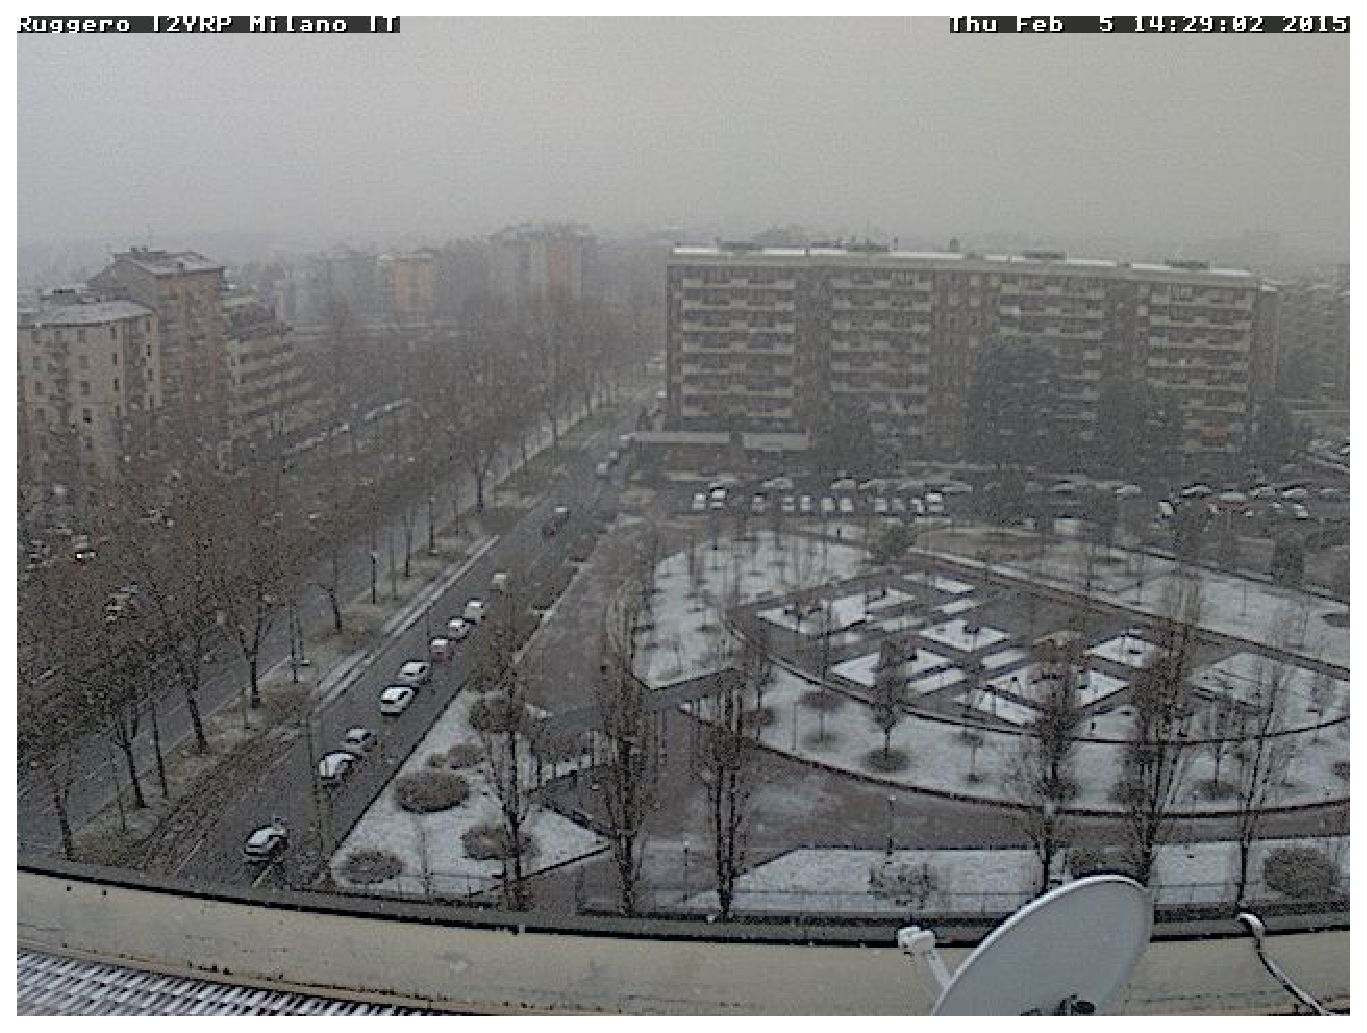
\includegraphics[width=6cm]{./pictures/testiORIGINALE}}
	\subfigure[]{\label{fig:displacementSPOSTATO}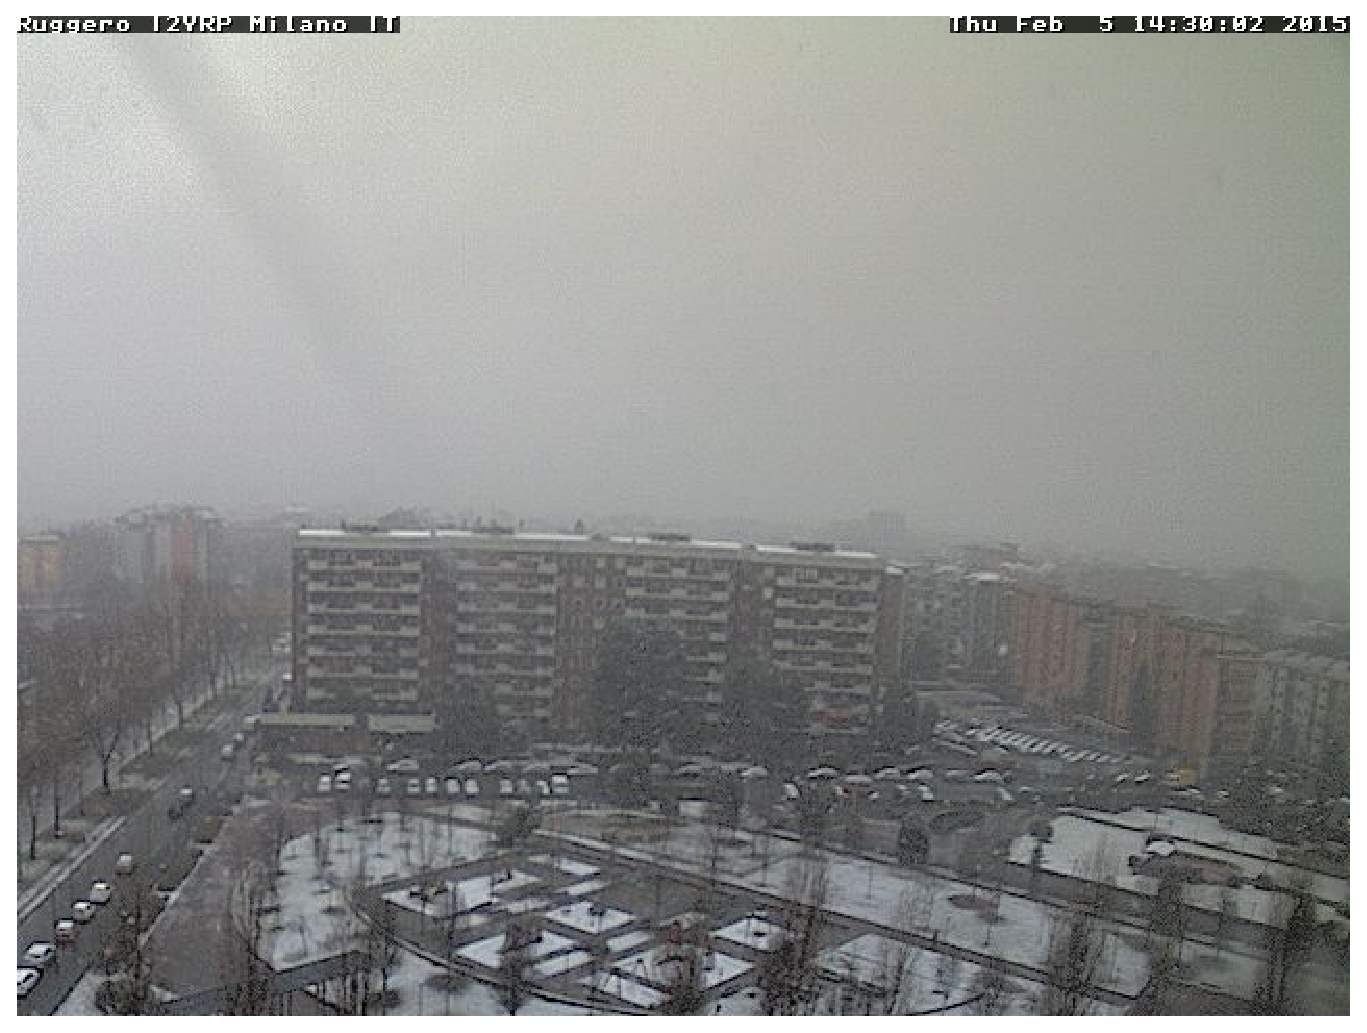
\includegraphics[width=6cm]{./pictures/testiDISPLACEMENT}}
	\caption{Esempio di spostamento della camera}
	\label{fig:testiDISPLACEMENT}
\end{figure}
\noindent Un esempio \`e mostrato nella Figura \ref{fig:testiDISPLACEMENT}, dove vediamo che tra il frame riportato in Figura \ref{fig:displacementORIGINALE} e quello in Figura \ref{fig:displacementSPOSTATO} c'\`e stato un evento che ha spostato la camera.
Possiamo formalizzare il concetto di spostamento della camera nel modo seguente: consideriamo la sequenza $\{y_t\}$ di immagini generate da una camera in una certa posizione, e la sequenza $\{w_t\}$ di immagini generate dalla stessa camera in una posizione differente.\\
Possiamo modellare la sequenza di immagini $\{z_t\}$ in cui avviene uno spostamento della camera all'istante $T^*$ nel seguente modo:
\begin{equation}
\label{eq:displacement}
z_t(x)  = \left\{ \begin{array}{rcl}
	y_t(x) + \eta(x) & \mbox{per} & t < T^* \\
	w_t(x) + \eta(x) & \mbox{per} & t \geqslant T^*
	\end{array}\right. ,
\end{equation}
dove $\eta(x)$ \`e un rumore stazionario.\\
In questa formulazione abbiamo considerato lo spostamento come un fenomeno \textit{istantaneo};
in generale, possiamo considerare una fase \textit{transitoria} in cui l'inquadratura della camera cambia a ogni \gls{frame} acquisito, fino a raggiungere la posizione finale. 
Dato che, nella nostra applicazione, la camera opera con \gls{framerate} molto bassi (come ad esempio un'immagine al minuto), possiamo considerare lo spostamento come istantaneo e, quindi, tenere come riferimento il modello \eqref{eq:displacement}.\\
%Nella formulazione pi\`u generale possiamo, quindi, assumere un istante $T_{start}^ *$ in cui inizia lo spostamento e un istante $T_{end}^*$ in cui termina il transitorio:
%\begin{equation}
%\label{eq:displacementGeneral}
%z_i(x) = \left\{ \begin{array}{rcl}
%y_i(x) + \eta(x) & \mbox{per} & i < T_{start}^* \\
%v_i(x) + \eta(x) & \mbox{per} & T_{start}^* \leq i < T_{end}^* \\
%w_i(x) + \eta(x) & \mbox{per} & i \geqslant T_{end}^*
%\end{array}\right. ,
%\end{equation}
%dove $\{v_i\}$ rappresenta la sequenza di immagini generate da viste differenti.
%Inoltre, durante il transitorio dello spostamento, il tempo di esposizione della camera pu\`o portare alla generazione di sfocature nelle immagini.\\
Anche per lo spostamento della camera vale la considerazione fatta nel caso della sfocatura: il contenuto delle immagini varia con il passare del tempo, quindi identificare lo spostamento confrontando frame consecutivi nel tempo genera un alto numero di falsi allarmi, come verr\`a mostrato dalla fase sperimentale.
\subsection{Occlusione e guasti della camera}
Il fenomeno dell'occlusione avviene quando un oggetto opaco si pone a ridosso della camera, impedendo la visione di una parte, se non la totalit\`a, della scena. 
\begin{figure}[tb]
	\centering
	\subfigure[]{\label{fig:occlusionCALZA} 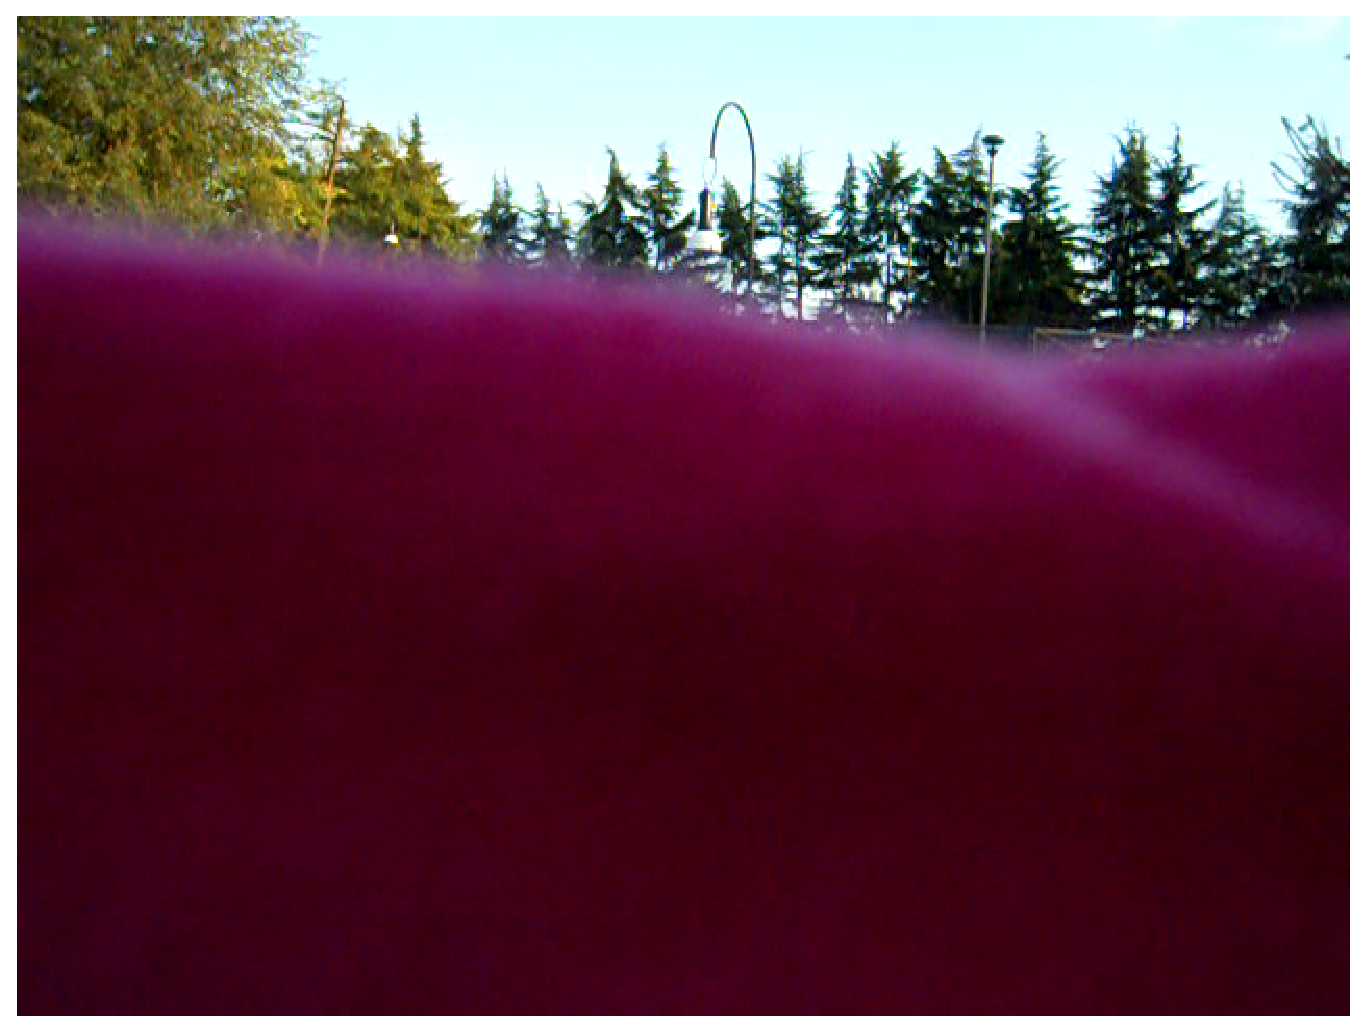
\includegraphics[width=6cm]{./pictures/calza}}
	\subfigure[]{\label{fig:occlusionNEVE}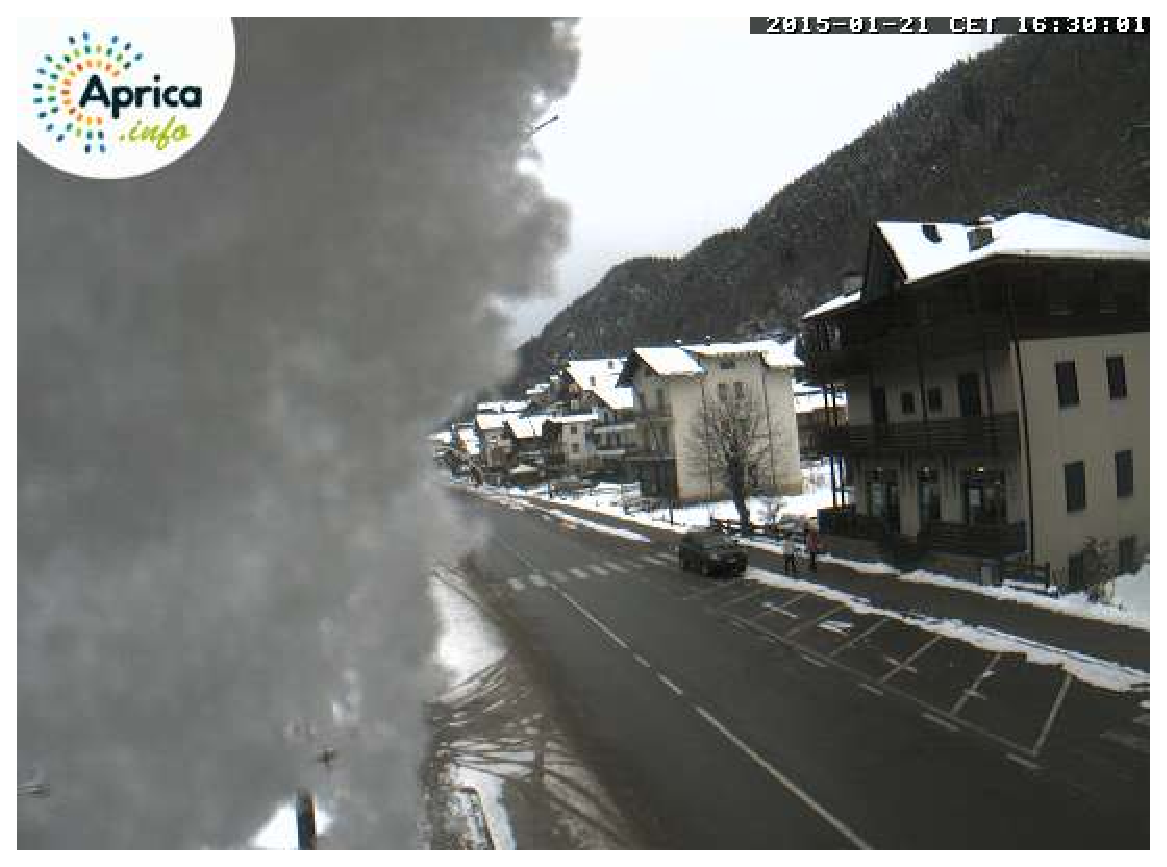
\includegraphics[width=6cm]{./pictures/neve}}
	\caption{Esempi di occlusione}
	\label{fig:occlusion}
\end{figure}
\noindent Esempi di occlusione sono illustrati in Figura \ref{fig:occlusion}. 
Pu\`o succedere (Fig. \ref{fig:occlusionCALZA}) che un oggetto venga posto intenzionalmente davanti alla lente della camera, in modo da coprire la scena, oppure (Fig. \ref{fig:occlusionNEVE}), a causa di una nevicata, pu\`o avvenire che della neve si depositi sulla lente e, quindi, venga compromessa la corretta acquisizione.\\
Quando parliamo di guasti, invece, possiamo considerare due casi:
\begin{itemize}
	\item guasto della \textit{trasmissione};
	\item guasto del \textit{sensore.}
\end{itemize}
Il primo caso pu\`o avvenire nel caso si considerino delle WMSN, in particolare quando i frame vengono trasmessi attraverso la rete dai sensori verso un nodo centrale.
Quando avviene un guasto nella rete parte dell'immagine non viene trasmessa, come illustrato nella Figura \ref{fig:guastoTrasmissione}.
Il caso del sensore guasto, come ad esempio quello nella Figura \ref{fig:guastoSensore}, comporta generalmente un aumento del rumore presente nel frame. \\
\begin{figure}[tb]
	\centering
	\subfigure[]{\label{fig:guastoTrasmissione} 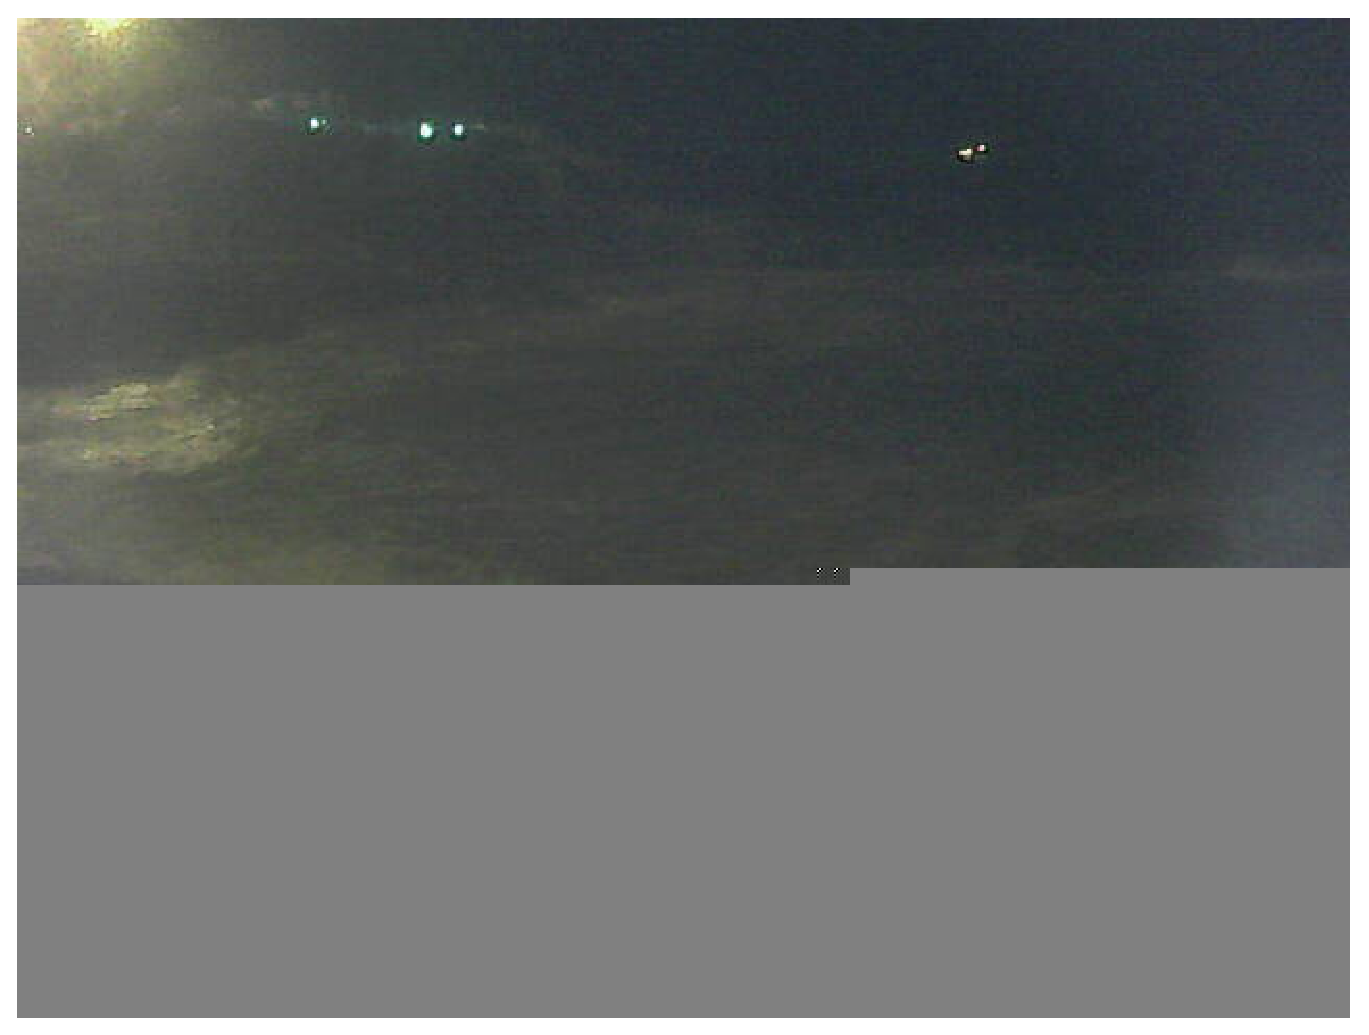
\includegraphics[width=6cm]{./pictures/erroreTrasm}}
	\subfigure[]{\label{fig:guastoSensore}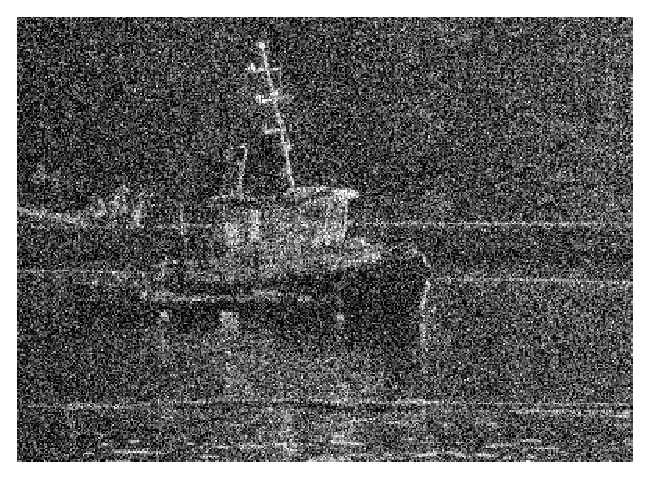
\includegraphics[width=6cm]{./pictures/rumore}}
	\caption[Esempi di guasti]{Esempi di guasti che possono compromettere l'acquisizione dei frame. In (a) vediamo un esempio di guasto della trasmissione, in cui parte dell'immagine non viene correttamente trasmessa nella rete. In (b), invece, vediamo un aumento del rumore nell'immagine, causato da un guasto del sensore della camera.}
	\label{fig:guasti}
\end{figure}
Questi problemi non sono stati affrontati durante il corso della tesi, comunque le tecniche messe a punto per rilevare spostamenti e sfocature possono essere utilizzate anche per rilevare questo tipo di eventi. 
\section{Tampering detection}
\label{tamperingDef}
Nel Paragrafo \ref{tamperingSOA} abbiamo introdotto in maniera molto generale il concetto di tampering detection. 
In questo paragrafo diamo una definizione pi\`u formale al problema.
L'algoritmo di tampering detection consiste nell'analizzare la sequenza dei frame generati dalla camera in modo da determinare un possibile cambiamento nell'inquadratura della scena o una sfocatura.\\
Consideriamo il caso generale di una sequenza di frame $\{z_t\}, t=1,\dots,\infty$. 
Per $t<T^*$ abbiamo che i frame vengono acquisiti in condizioni di funzionamento normale:
\[ z_t(x)=y_t(x) + \eta(x), \forall x \in \mathcal{X} \mbox{, per } t=1,\dots , T^*-1. \] 
All'istante di tempo $t = T^*$ avviene un evento di tampering, il quale compromette i frame per $t\geq T^*$.  
In particolare, nel caso di una sfocatura avremo
\[ z_t = \mathcal{B}_t[y_t](x) + \eta(x), \forall x \in \mathcal{X} \mbox{, per } t \geq T^*,\]
mentre nel caso di uno spostamento della camera avremo
\[ z_t = w_t(x) + \eta(x), \forall x \in \mathcal{X} \mbox{, per } t \geq T^*. \]
%Nel caso dell'operatore di degradazione $\mathcal{D}$, con riferimento al modello descritto nell'equazione \eqref{blur_multi}, possiamo considerare che, in condizioni di funzionamento normale, l'operatore di sfocatura $\mathcal{B}$ si comporti come un \textit{filtro passa-tutto}, ovvero
%\[\mathcal{B}_i[y](x)=y_i(x) \mbox{, per } i=1,\dots, T^*,\]
%e che all'istante $T^*$ esso cambi, diventando come nel caso dell'equazione \eqref{eq:blur}.
L'obiettivo dell'algoritmo di tampering detection \`e quello di stimare l'istante $T^*$. \\
%Nel caso dell'operatore di spostamento $\mathcal{S}$, tenendo come riferimento la formula \eqref{eq:displacement}, l'obiettivo dell'algoritmo \`e quello di stimare l'istante di tempo $T^*$ in cui avviene il passaggio dalla sequenza di immagini $\{y_i\}$ a $\{w_i\}$.\\
Come abbiamo illustrato precedentemente, discriminare tra cambiamenti avvenuti a livello di contenuto della scena e cambiamenti dovuti a tampering pu\`o diventare complicato confrontando direttamente i frame tra loro, in quanto stiamo operando con framerate bassi.
%Non \`e, quindi, possibile utilizzare le tecniche basate su background che sono state descritte nel paragrafo \ref{background}.
Non utilizzeremo, quindi, le tecniche basate su background che sono state descritte nel Paragrafo \ref{background}.
Nel Capitolo \ref{SoluzioneProposta} vedremo la soluzione che abbiamo deciso di utilizzare per lo sviluppo dell'algoritmo di tampering detection. 